\chapter{Monitoring layer}\label{G:monitoringLayer}

As already discussed, in order to properly manage a cloud computing environment it is strongly required to use monitoring tools in order to gather information of interest by improving the environment itself or by finding out issues and solving them as fast as possible.

This chapter aims to showcase how the selected monitoring tools can fit in the architecture type that has been proposed. And, how they can be used. This means, preparing the environment to support Collectd (i.e.: monitoring and gathering) and Graphite (i.e.: storing and presenting) tools.

Moreover, to point out that such tools are helpful to demonstrate that LiveMediaStreamer framework could be deployed as the core of a real-time media production platform (see chapter \ref{H:platformDeploymentAndDemonstrations}).

So, to remark that the fact of creating small and reusable containers is the main goal of this chapter and, of course, the goal of this platform architecture to prototype. And, thanks to the selected monitoring tools, which are lightweight and ease configuration flexibility, this issue might be properly solved.

Then, a proposal of the monitoring architecture in a more detailed description (regarding figure \ref{F:MLAP}) is shown in figure \ref{F:maex}.

\begin{figure}[htb]
\begin{center}
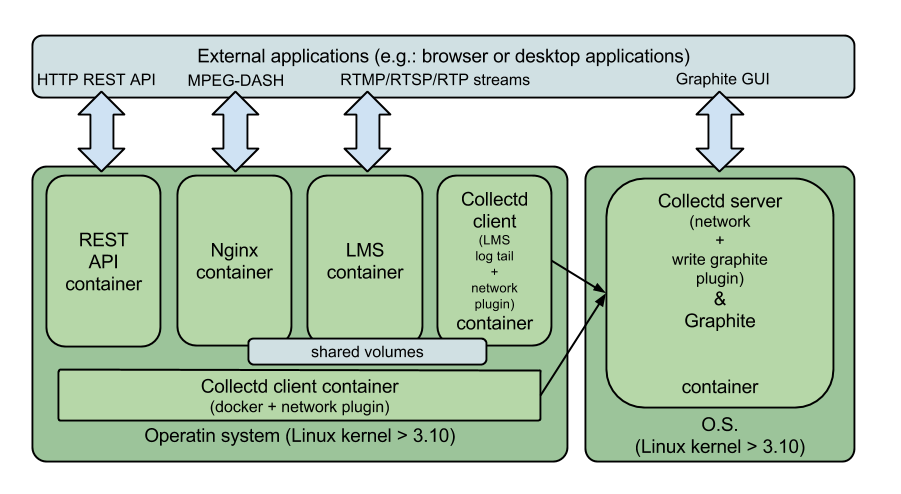
\includegraphics[width=0.9\textwidth]{./images/monitArchProp.png}
\caption{Detailed monitoring architecture}
\label{F:maex}
\end{center}
\end{figure}

Figure \ref{F:maex} showcases the relationship between different containers and the whole Collectd+Graphite deployment. Following sections are explaining it:

\section{Monitoring containers}

This section is based on how Collectd can be configured and deployed in order to monitor and properly gather metrics of interest.

\subsection{From O.S. point of view}

The fact of using Collectd means a wide community behind, which probably have already developed required functionalities (i.e.: plugins). And this is the case: in order to monitor each of the containers that a host O.S. might have it can be solved by configuring already existing plugins for Collectd from Docker community. 

The selected plugin is using the stats API introduced since Docker 1.5 version. And, concretely, the reported container's stats are:
 
\begin{itemize}
\item Network bandwidth
\item Memory usage
\item CPU usage
\item Block IO
\end{itemize}

The pluguin is called "docker-collectd-pluguin" and can be found in \href{https://github.com/lebauce/docker-collectd-plugin}{GitHub} (--REFERENCE--).

Therefore, the O.S. system requires having a basic collectd daemon running and to be configured in order to send gathered metrics to a centralized collectd server (as proposed in figure \ref{F:maex}).

So, from O.S. point of view, next example of this specific Collectd's plugins configuration showcases how to load and configure such plugins:

\begin{verbatim}

TypesDB "/usr/share/collectd/docker-collectd-plugin/dockerplugin.db"
LoadPlugin python

<Plugin python>
  ModulePath "/usr/share/collectd/docker-collectd-plugin"
  Import "dockerplugin"

  <Module dockerplugin>
    BaseURL "unix://var/run/docker.sock"
    Timeout 3
  </Module>
</Plugin>

LoadPlugin network
<Plugin network>
  Server "graphite-host-address" "graphite-host-port"
  ReportStats true
</Plugin>

\end{verbatim}

Previous Collectd configuration file sets the python (i.e.: docker-collectd-plugin) plugin as an input from the O.S. Docker API daemon and the network plugin as an output to the Collectd server.

\subsection{From container point of view}

From a container point of view and by following the premise to build containers as reusable as possible what is proposed to implement is a container that has the goal to gather the logged stats from an LMS container. This, as shown in figure \ref{F:maex}, implies sharing a Docker volume (as introduced in previous chapter \ref{D:virtualization}) from LMS container to the Collectd client which is using the tail plugin as an input. Moreover, in order to send specific logged metrics to the Collectd server container it is also using the network plugin as done in previous Collectd client configuration.

But, first of all, it is also required to be built in a container. So, this is the Docker file:

\begin{verbatim}

FROM    ubuntu:14.04
MAINTAINER Gerard CL <gerardcl@gmail.com>

ENV     DEBIAN_FRONTEND noninteractive

RUN apt-get update
RUN apt-get -y install collectd curl python-dev python-pip

ADD collectd.conf.tpl /etc/collectd/collectd.conf.tpl

RUN pip install envtpl
ADD start_container /usr/bin/start_container
RUN chmod +x /usr/bin/start_container
CMD start_container

\end{verbatim}

The, what is done in this case is to specify a bash script to run as CMD. This runs collectd but after envtpl python's package sets the environment parameters:
\begin{verbatim}
#!/bin/bash
envtpl /etc/collectd/collectd.conf.tpl
collectd -C /etc/collectd/collectd.conf -f
\end{verbatim}

Thanks to the envtpl package it is possible to run the container with specific environment variables in order to configure following parameters:

\begin{itemize}
\item LMS NAME \hfill

this will be used to identify the LMS instance in a container which Collectd is monitoring.
\item GRAPHITE HOST \hfill

this is to set the address of the remote/local container where the Collectd server is listening and pushing the metrics inside the Graphite's tools.
\item GRAPHITE PORT \hfill

this is the port where the Collect server and Graphite's tools container is listening to.
\end{itemize}

And these parameters are set in the Collectd configuration file as shown next (among the specific plugins):

\begin{verbatim}
Hostname "{{ LMS_NAME }}"
FQDNLookup true

Interval 1
Timeout 4
ReadThreads 5

LoadPlugin syslog
LoadPlugin cpu
LoadPlugin load
LoadPlugin memory
LoadPlugin network

<Plugin "syslog">
  LogLevel "info"
  NotifyLevel "OKAY"
</Plugin>

<Plugin network>
  Server "{{ GRAPHITE_HOST }}" "{{ GRAPHITE_PORT | default("25826") }}"
  ReportStats true
</Plugin>
\end{verbatim}

This Collectd configuration example file is loading specific system loggers plugins as inputs to be sent through the network plugin to the Collectd server.

But, in next chapter \ref{H:platformDeploymentAndDemonstrations} is shown an example of use of the Collectd tail plugin by using regular expressions. And this, as shown in figure \ref{F:maex}, this tail plugin is listening in an specific folder which is shared through the Docker's volume functionality with the LMS container, which logs its metrics in the same volume.

Finally, the Docker run command where the specific environment variables are set should be as shown next:
\begin{verbatim}
$ docker run -it -e "LMS_NAME=lms" \
	-e "GRAPHITE_HOST=<IP address>" -e "GRAPHITE_PORT=25826" \
	--rm --name cdc \
	-p 25826:25826/udp gerardcl/lms-collectd-client
\end{verbatim}

This will start immediately sending the defined container stats to the Graphite container specified by the environment parameters. Following section showcases the Graphite side to be deployed.

So, this example of deployed container for isolated Collectd clients is a key point in the general monitoring architecture due to the fact of being easyly configurable and reusable.

\section{Showcasing monitoring}

container amb graphite + collectd server

mostrar com es genera tot (referències a fitxers externs??) i imatges del graphite o escenari sencer. amb exemples concrets mostrant potencial de graphite!!!

This section is focused on the storage and presentation side of the metrics already logged and gathered.

So, as already introduced, this is proposed to be done within a container built with a Collectd server (network data inputs served to Graphite) and a Graphite system (storing and presenting stats).

As commonly said by the Collectd and Graphite community, installing and configuring Graphite isn't at all so easy than installing and configuring Collectd. This fact is shown in the following Docker file in order to build such container, as shown in figure \ref{F:maex}:

\begin{verbatim}
# LiveMediaStreamer Container
FROM ubuntu:14.04
MAINTAINER Gerard CL <gerardcl@gmail.com>

RUN apt-get update
RUN apt-get install -y python-cairo collectd-core libgcrypt11 \
python-virtualenv build-essential python-dev supervisor sudo

RUN adduser --system --group --no-create-home collectd \
&& adduser --system --home /opt/graphite graphite

RUN sudo -u graphite virtualenv --system-site-packages ~graphite/env

RUN echo "django \n \
  python-memcached \n \
  django-tagging \n \
  twisted \n \
  gunicorn \n \
  whisper \n \
  carbon \n \
  graphite-web" > /tmp/graphite_reqs.txt

RUN sudo -u graphite HOME=/opt/graphite /bin/sh -c ". \
~/env/bin/activate && pip install -r /tmp/graphite_reqs.txt"

ADD collectd/collectd.conf /etc/collectd/
ADD supervisor/ /etc/supervisor/conf.d/
ADD graphite/settings.py /opt/graphite/webapp/graphite/
ADD graphite/local_settings.py /opt/graphite/webapp/graphite/
ADD graphite/mkadmin.py /opt/graphite/webapp/graphite/
ADD graphite/storage-schemas.conf /opt/graphite/conf/

RUN cp /opt/graphite/conf/carbon.conf.example \
/opt/graphite/conf/carbon.conf
RUN cp /opt/graphite/conf/graphite.wsgi.example \
/opt/graphite/webapp/graphite/graphite_wsgi.py
RUN cp /opt/graphite/conf/graphite.wsgi.example \
/opt/graphite/conf/graphite.wsgi
RUN cp /opt/graphite/conf/storage-aggregation.conf.example \
/opt/graphite/conf/storage-aggregation.conf

RUN sed -i "s#^\(SECRET_KEY = \).*#\1\"`python -c 'import os; import base64; \
print(base64.b64encode(os.urandom(40)))'`\"#" \
/opt/graphite/webapp/graphite/app_settings.py
RUN sudo -u graphite HOME=/opt/graphite PYTHONPATH=/opt/graphite/lib/ \
/bin/sh -c "cd ~/webapp/graphite && ~/env/bin/python manage.py syncdb --noinput"
RUN sudo -u graphite HOME=/opt/graphite PYTHONPATH=/opt/graphite/lib/ \
/bin/sh -c "cd ~/webapp/graphite && ~/env/bin/python mkadmin.py"

EXPOSE 8080 25826/udp

CMD exec supervisord -n
\end{verbatim}

In this case, specific "collectd" and "graphite" users are created (among other environment configurations as shown).
Then, a bunch of different and specific configuration files for graphite are added (i.e.: ADD command) to their specific configuration folders. And, finally, specific command executions for database synchronization (sqlite3) and other final configurations required for Graphite are also done (--REFERENCE-- intalling graphite). Regarding Collectd, it is installed in a similiar way as previously done but it is now configured as follows:

\begin{verbatim}
Hostname "localhost"
FQDNLookup true
Interval 1

LoadPlugin syslog
LoadPlugin network
LoadPlugin write_graphite

<Plugin syslog>
	LogLevel "info"
	NotifyLevel "OKAY"
</Plugin>

<Plugin network>
	Listen "*" "25826"
	ReportStats true
</Plugin>

<Plugin write_graphite>
	<Node "graphing">
		Host "localhost"
		Port "2003"
		Protocol "tcp"
		LogSendErrors true
		Prefix "collectd."
		StoreRates true
		AlwaysAppendDS false
		EscapeCharacter "_"
	</Node>
</Plugin>
\end{verbatim}

So, here, Collectd is configured as a server by listening from anywhere at the default port for Collectd clustering. Moreover, the "write graphite" plugin is loaded in order to work as an output to the Graphite's Carbon tool, which receives the data to be stored in the Whisper RRD of the Graphite installation.

In this case, it is required to configure this container to be able to run multiple processes (i.e.: Graphite and Collectd). Therefore, by following previous section of how to run multiple processes inside a container in chapter \ref{D:virtualization}, the Supervisord system is used. This time it's configured by splitting the processes configurations into two parts, the Collectd and the Graphite. This last is configuring the Graphite web application and the Graphite's Carbon cache.

\begin{itemize}
\item Collectd: \hfill

\begin{verbatim}
[program:collectd]
user=collectd
directory=/
command=collectd -C /etc/collectd/collectd.conf -f
stdout_logfile=/var/log/supervisor/%(program_name)s.log
stderr_logfile=/var/log/supervisor/%(program_name)s_error.log
\end{verbatim}
\item Graphite web: \hfill

\begin{verbatim}
[program:graphite-web]
user=graphite
directory=/opt/graphite/webapp/
command=/opt/graphite/env/bin/gunicorn -w 1 -b 0.0.0.0:8080 \
	--pythonpath /opt/graphite/webapp/graphite graphite_wsgi
stdout_logfile=/var/log/supervisor/%(program_name)s.log
stderr_logfile=/var/log/supervisor/%(program_name)s_error.log
\end{verbatim}

\item Carbon cache: \hfill

\begin{verbatim}
[program:carbon-cache]
user=graphite
directory=/
env=PYTHONPATH=/opt/graphite/lib/
command=/opt/graphite/bin/carbon-cache.py --debug start
stdout_logfile=/var/log/supervisor/%(program_name)s.log
stderr_logfile=/var/log/supervisor/%(program_name)s_error.log
\end{verbatim}
\end{itemize}

An important configuration that must be decided and configured by knowing the requirements for why monitoring is required implies defining the storage schemas, which detail retention rates for storing metrics by following what was introduced in chapter \ref{B:problemStatementAndProposal}, the Round-Robin Database storage type. So, in order to work over a real-time media production platform it is important to achieve as much time accuracy as possible regarding the specific metrics of interest (e.g.: bandwidth usage, losses, pipeline delays, \ldots). There are more files regarding the Graphite's tools configuration (see APPENDIX XXX) too, but most of them are set to default values which are the recommended ones. 

Before going to present results and comment the outcomes (chapter \ref{H:platformDeploymentAndDemonstrations}), it is important to showcase example commands for both Collectd client and Collectd server + Graphite's containers:

\begin{verbatim}
$ docker run -it -e "LMS_NAME=lms" -e "GRAPHITE_HOST=<IP of >" \
--rm --name collectd -p 25826:25826/udp gerardcl/lms-collectd-client
\end{verbatim}

\begin{verbatim}
$ docker run -it --rm --name graphite -p 25826:25826/udp -p 8080:8080 \
gerardcl/lms-collectd-graphite
\end{verbatim}

As shown, the collectd (i.e.: Collectd client) container is sending to the default port (i.e.: UDP protocol) of the graphite host's (Collectd server and Graphite tools) container. Moreover, the graphite container opens HTTP port 8080 in order to enable browsers to get access to its web application anywhere. 